\documentclass[11pt,a4paper]{article}
\usepackage[utf8]{inputenc}
\usepackage[T1]{fontenc}
\usepackage{geometry}
\usepackage{amsmath,amssymb,amsfonts}
\usepackage{graphicx}
\usepackage{booktabs}
\usepackage{hyperref}
\usepackage{microtype}
\usepackage{float}
\usepackage[section]{placeins}


\geometry{left=25mm,right=25mm,top=25mm,bottom=25mm}

\hypersetup{
    colorlinks=true,
    linkcolor=blue,
    filecolor=magenta,      
    urlcolor=cyan,
    citecolor=blue,
}

\title{\textbf{Optimal Integrated Control of Suspension Damping and Braking for Minimum Braking Distance}}
\author{Ivan Valiant Susanto \\ 
\small Master's Programme in Vehicle Engineering \\ 
\small KTH Royal Institute of Technology, Stockholm, Sweden}
\date{\today}

\begin{document}

\maketitle

\begin{abstract}
Traditional vehicle braking and suspension systems are typically designed and controlled in isolation. However, the maximum longitudinal braking force a tire can transmit is strictly bounded by the dynamic normal load ($F_x \le \mu F_z$). During transient braking maneuvers (brake dive), normal loads fluctuate significantly. This project investigates the theoretical and simulation-based potential of synchronously and continuously co-optimizing semi-active/active suspension damping and braking forces to actively manage transient load transfer and minimize braking distance. The work establishes a foundational study using an analytical 2-DOF half-car model (sprung mass heave and pitch) with a structured pathway for scaling to a 4-DOF model (incorporating unsprung masses), progressing through a hierarchical tire model progression (Linear, Nonlinear Saturation, Brush, and Magic Formula 6.2 via \texttt{mfeval}), and culminating in high-fidelity multi-body validation using CarSim.
\end{abstract}

\section{Introduction and Background}
During emergency or performance braking, vehicle pitch dynamics—commonly known as ``brake dive''—cause a forward shift in axle load distribution. While static load transfer is governed by vehicle geometry and center of gravity height, the *transient* peak normal load can be actively influenced by controlling suspension damping forces. 

Standard anti-dive suspension geometries or decoupled control systems often compromise ride comfort or peak deceleration response because they cannot adaptively sculpt transient normal loads. By treating damping and braking as a unified mechatronic control problem, this thesis explores how optimal control algorithms can exploit tire friction limits more effectively to shorten braking distances.

\section{Research Objectives and Scope}
The primary objective of this thesis is to quantify the performance ceiling of integrated suspension and brake control during straight-line braking. The project scope is defined by the following key objectives:
\begin{itemize}
    \item \textbf{Mathematical Modeling:} Formulate an initial linear 2-DOF half-car state-space model capturing sprung mass vertical bounce (heave, $z$) and pitch ($\theta$), with subsequent expansion capability to a 4-DOF model including front and rear unsprung masses.
    \item \textbf{Tiered Tire Modeling:} Implement progressive tire dynamics, starting from linear approximations, moving to nonlinear friction saturation limits, semi-analytical brush models, and finalizing with Pacejka Magic Formula 6.2 via the \texttt{mfeval} toolbox.
    \item \textbf{Control Synthesis \& Benchmarking:} Design and evaluate optimal controllers (e.g., LQR, MPC) alongside classical rule-based strategies (e.g., Groundhook damping) and robust frameworks ($H_\infty$).
    \item \textbf{Multi-Body Co-Simulation:} Validate custom MATLAB/Simulink control architectures against high-fidelity vehicle plants using CarSim (leveraging host company simulation licenses).
\end{itemize}

\section{Methodology and Simulation Framework}
\subsection{Half-Car State-Space Formulation and Actuator Realization}
To facilitate optimal control design and provide a transparent preliminary demo, the initial phase starts with a 2-DOF model neglecting unsprung mass hop to isolate low-frequency body dynamics (1--3 Hz). The equations of motion for sprung mass heave ($m\ddot{z}$) and pitch ($I_y\ddot{\theta}$) are expressed in state-space form:
\begin{equation}
    \dot{x}(t) = A x(t) + B u(t) + W w(t)
\end{equation}
\begin{equation}
    y(t) = C x(t) + D u(t)
\end{equation}
where the state vector $x = \begin{bmatrix} z & \theta & \dot{z} & \dot{\theta} \end{bmatrix}^T$ contains body displacements and velocities, and the control input vector $u = \begin{bmatrix} F_{df,\text{req}} & F_{dr,\text{req}} \end{bmatrix}^T$ represents the ideal damping forces computed by the LQR synthesis. 

To account for physical hardware limitations, these ideal LQR control forces are not applied directly to the plant. Instead, they pass through a \textit{Clipped Optimal Control} realization layer that enforces semi-active passivity ($F_d \cdot \dot{x}_{\text{rel}} \le 0$), damping coefficient saturation ($c_{\min} \le c \le c_{\max}$), and solenoid valve bandwidth limits via slew-rate constraints. The disturbance vector $w$ accounts for longitudinal deceleration pitch moments. Subsequent phases expand this framework into a \textbf{4-DOF model} by incorporating front and rear wheel unsprung masses ($z_{uf}, z_{ur}$) to capture high-frequency wheel-hop interactions.

\subsection{Tire Dynamics Progression}
To accurately capture the interaction between normal load transfer and force saturation, the simulation framework utilizes a structured four-tier tire model hierarchy:
\begin{enumerate}
    \item \textbf{Linear Tire Model:} Used for initial controller tuning and analytical validation under small slip assumptions.
    \item \textbf{Nonlinear Friction Saturation Model:} Imposes fundamental friction limits ($F_{x,\max} = \mu F_z$) to observe load-coupling effects on braking force limits.
    \item \textbf{Brush Tire Model:} Introduces adhesion and sliding physics to study semi-analytical nonlinear force generation.
    \item \textbf{Pacejka Magic Formula 6.2 (\texttt{mfeval}):} Deploys industry-standard empirical equations via MATLAB's \texttt{mfeval} toolbox to evaluate performance under realistic combined slip and tire characteristics.
\end{enumerate}

\subsection{Toolchain and Co-Simulation}
\begin{itemize}
    \item \textbf{MATLAB/Simulink:} Primary environment for analytical derivation, matrix parameterization, tire evaluation via \texttt{mfeval}, and optimal controller synthesis.
    \item \textbf{CarSim:} Utilized for advanced multi-body vehicle plant validation, cross-checking custom Simulink algorithms against industry-standard vehicle dynamics software using corporate license infrastructure.
\end{itemize}

\section{Scope Limitations and Future Development}
While this study isolates the co-optimization of suspension damping and global braking force to maximize normal load ($F_z$) during transient brake dive, real-world implementation must interface with tire slip limits. 

\begin{itemize}
    \item \textbf{Exclusion of ABS Optimization:} High-frequency wheel slip control (ABS operating at $15\text{--}50+\text{ Hz}$) is deliberately decoupled from low-frequency suspension pitch dynamics ($1\text{--}3\text{ Hz}$) to maintain a focused thesis scope.
    \item \textbf{Future Extension:} Future iterations of this framework could integrate a slip-based braking controller layer to simultaneously optimize normal load transfer and tire slip ratio, achieving a fully integrated chassis control architecture.
\end{itemize}

\section{Preliminary Simulation Results and Tire-Braking Co-Simulation}
To validate the 2-DOF half-car state-space framework under realistic hardware limitations, an initial simulation was conducted comparing a passive baseline damper to the proposed semi-active LQR controller. An overview of the closed-loop Simulink architecture is detailed in Appendix~A (Figure~\ref{fig:main_sim}).

The semi-active implementation integrates three core Öhlins solenoid valve constraints (further illustrated in Appendix~A, Figure~\ref{fig:damper_model}):
\begin{enumerate}
    \item \textbf{Damping Coefficient Saturation:} Bounded between $c_{\min} = 500\text{ N}\cdot\text{s/m}$ and $c_{\max} = 4000\text{ N}\cdot\text{s/m}$.
    \item \textbf{Passivity Constraint:} Enforced via velocity-guard logic ensuring the damper remains purely dissipative ($F_d \cdot \dot{x}_{\text{rel}} \le 0$), preventing any external energy injection.
    \item \textbf{Valve Bandwidth Limits:} Modeled using a slew-rate limiter to simulate solenoid response lag during transient events.
\end{enumerate}

To evaluate the cross-coupling between suspension pitch dynamics and longitudinal braking, a \textbf{Tier 2 Non-Linear Friction Saturation model} ($F_{x,\max} = \mu F_z$) was incorporated via custom Simulink subsystems (depicted in Appendix~A, Figures~\ref{fig:tire_passive} and \ref{fig:tire_semi}). 

Under low-friction conditions ($\mu = 0.4$), the limitations of transient load transfer become critical. As detailed in Table~\ref{tab:prelim_results} and visualized in Figure~\ref{fig:result1}, the semi-active LQR controller successfully suppresses transient body motion during a braking maneuver. By aggressively cutting down oscillation peaks during the initial transient phase, the controller stabilizes the vertical normal loads ($F_z$), preventing premature tire force clipping at the saturation boundary. 

Consequently, as shown in Figure~\ref{fig:acc_result}, the semi-active configuration achieves higher sustained deceleration ($a_x$) compared to the under-damped passive baseline. While this higher braking force results in a marginally deeper steady-state nosedive due to increased load transfer ($\Delta F_z = \frac{m h a_x}{L}$), the transient overshoot and settling behavior are vastly superior.

\begin{figure}[!htbp]
    \centering
    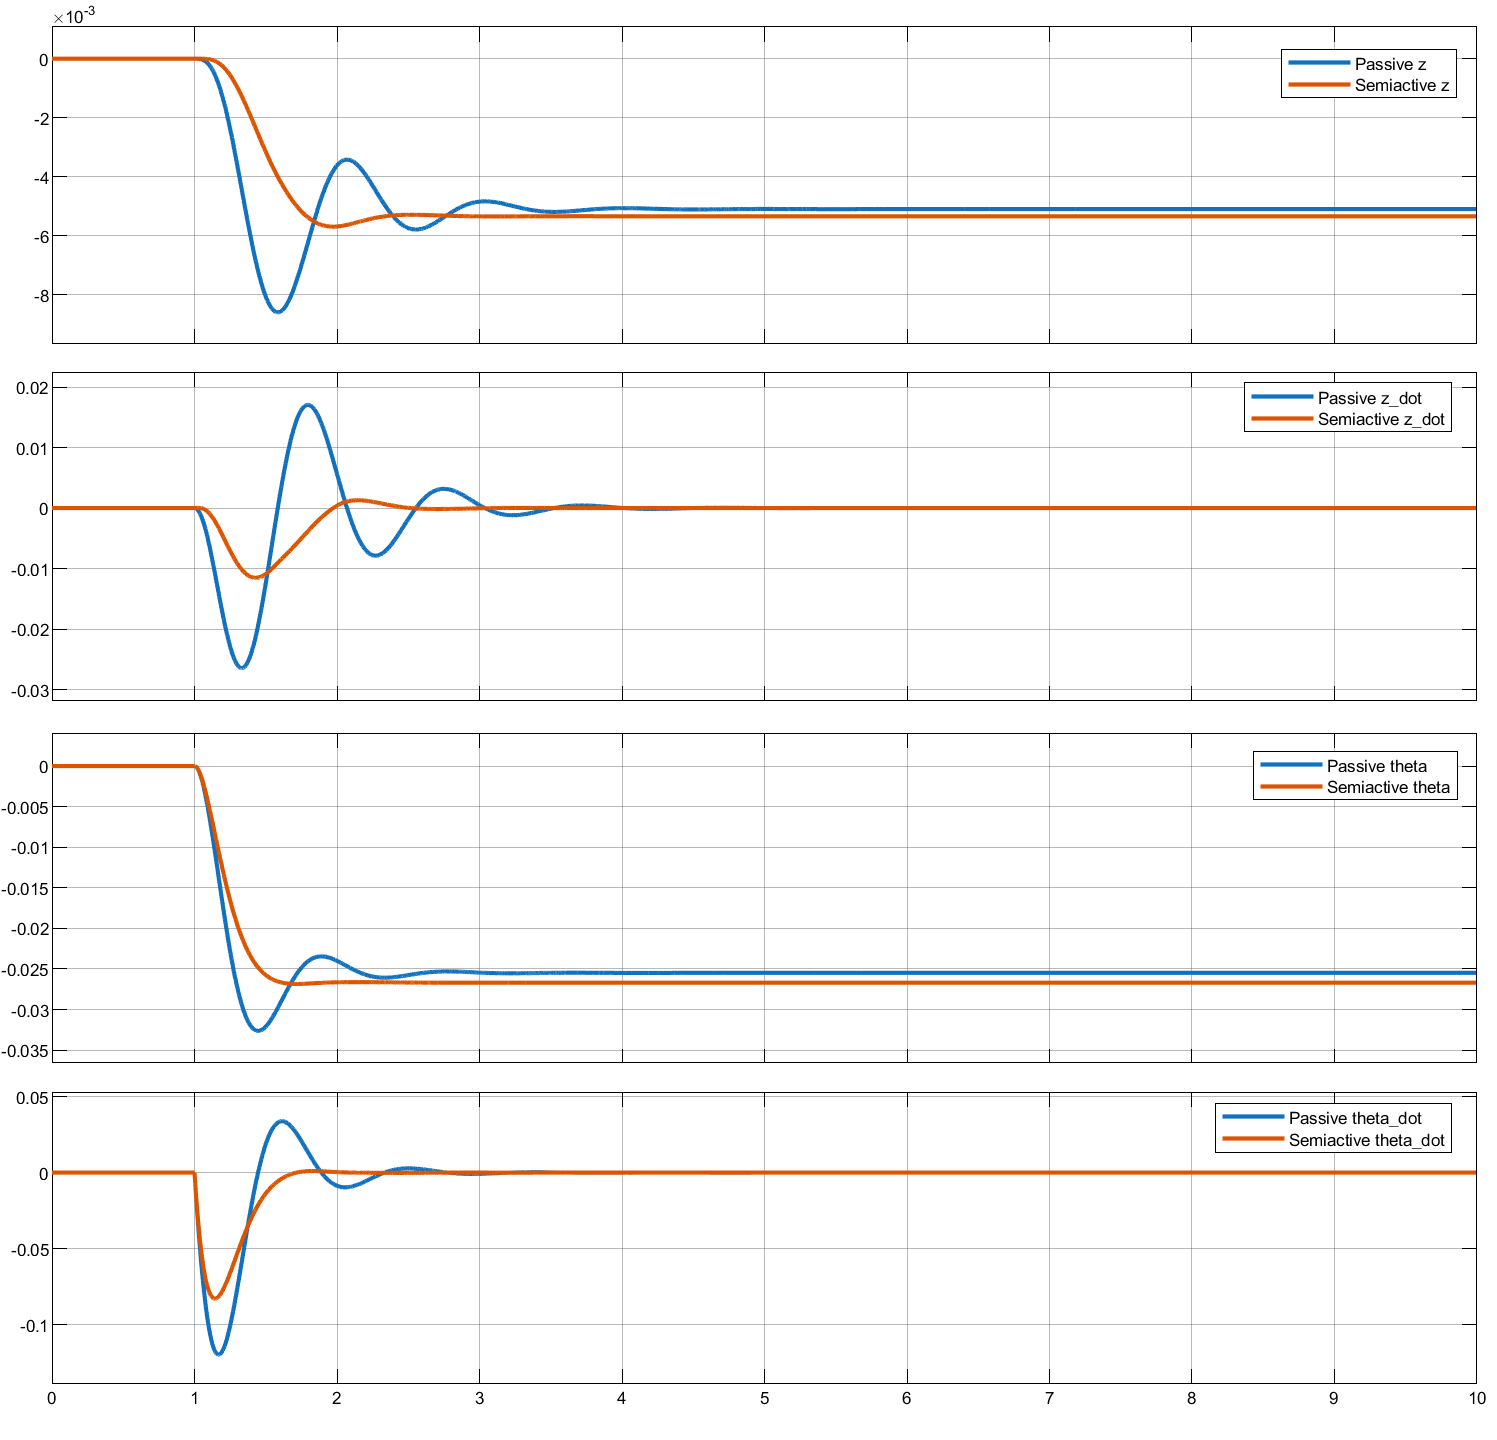
\includegraphics[width=0.85\textwidth]{result1.png}
    \caption{Simulation scope comparison (Passive vs. Semi-Active LQR under $\mu = 0.4$) highlighting the reduction in transient pitch and heave oscillations.}
    \label{fig:result1}
\end{figure}

\begin{figure}[!htbp]
    \centering
    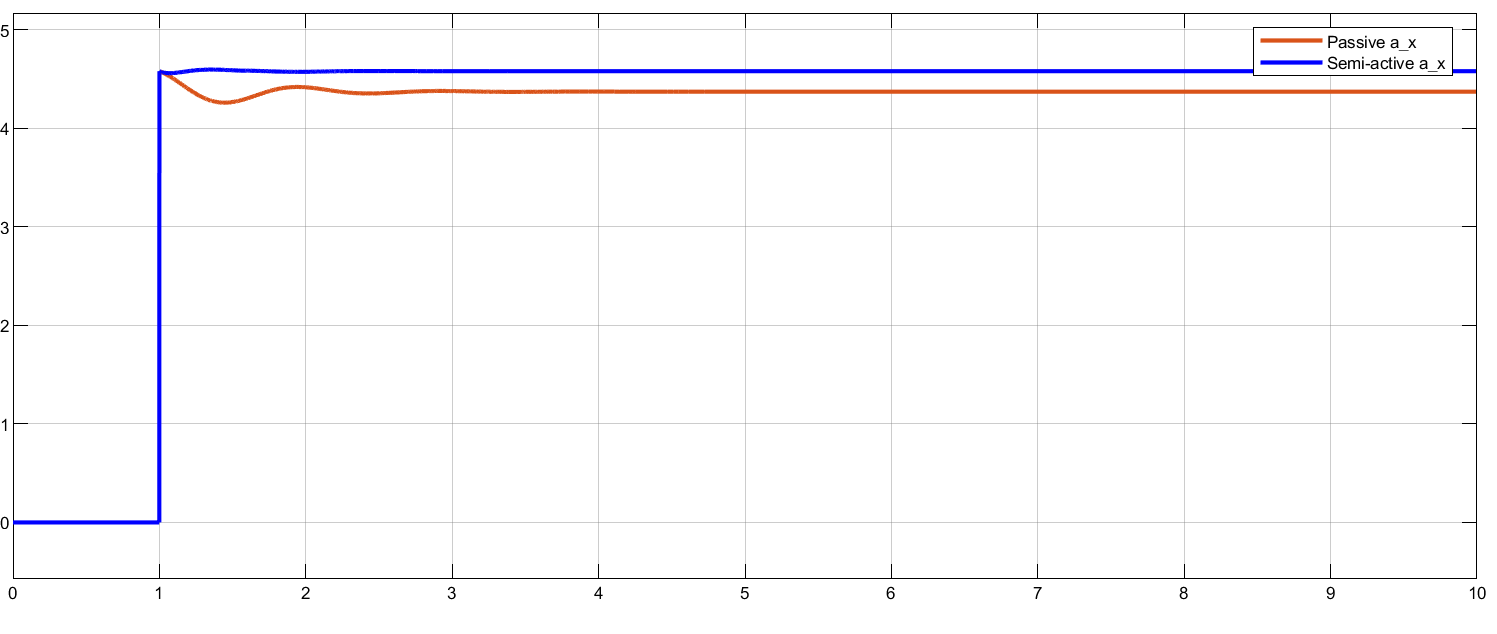
\includegraphics[width=0.85\textwidth]{acc_result.png}
    \caption{Longitudinal deceleration ($a_x$) comparison showing the semi-active controller sustaining higher braking performance by avoiding tire saturation.}
    \label{fig:acc_result}
\end{figure}

\begin{table}[!h]
\centering
\caption{Quantitative Comparison of Transient Braking Performance ($\mu = 0.4$, Passive vs. Semi-Active LQR)}
\label{tab:prelim_results}
\begin{tabular}{lccc}
\toprule
\textbf{Kinematic Metric} & \textbf{Passive Baseline} & \textbf{Semi-Active LQR} & \textbf{Peak Reduction (\%)} \\
\midrule
Heave ($z$) [m] & 0.00859 & 0.00569 & 33.77\% \\
Heave Velocity ($\dot{z}$) [m/s] & 0.02645 & 0.01152 & 56.44\% \\
Pitch Angle ($\theta$) [rad] & 0.03263 & 0.02685 & 17.72\% \\
Pitch Velocity ($\dot{\theta}$) [rad/s] & 0.11981 & 0.08293 & 30.78\% \\
\bottomrule
\end{tabular}
\end{table}


\section{Proposed Timeline and Milestones}
The research and development schedule is structured across five progressive phases, moving from analytical modeling to physical co-simulation:

\begin{table}[H]
\centering
\caption{Project Milestones and Estimated Timeline}
\label{tab:timeline}
\begin{tabular}{lll}
\toprule
\textbf{Phase} & \textbf{Task Description} & \textbf{Timeframe} \\
\midrule
Phase 1 & Literature review, 2-DOF derivation, and linear/nonlinear tire setup in MATLAB & Weeks 1--3 \\
Phase 2 & Implementation of Brush and Magic Formula (\texttt{mfeval}) tire models & Weeks 4--6 \\
Phase 3 & Advanced control design (LQR/MPC/Groundhook) and 4-DOF expansion & Weeks 7--10 \\
Phase 4 & CarSim multi-body integration, actuator bandwidth limits, and uneven roads & Weeks 11--13 \\
Phase 5 & Final analysis, report writing, and presentation preparation & Weeks 14--16 \\
\bottomrule
\end{tabular}
\end{table}

\section{Expected Deliverables}
Upon completion of this research project, the primary deliverables will include:
\begin{enumerate}
    \item A modular, well-documented MATLAB/Simulink and CarSim co-simulation framework.
    \item A comprehensive thesis report analyzing trade-offs between braking distance minimization, ride quality, and actuator constraints across progressive tire models.
    \item Quantitative performance metrics providing actionable insights for advanced suspension development.
\end{enumerate}

\section*{Transparency and AI Tool Disclosure}
In accordance with modern academic and professional research standards, generative AI tools (such as large language models) were consulted during the preparation of this proposal for structural outlining, editorial refinement, and syntax assistance in script development. All technical modeling choices, mathematical formulations, control strategy selections, and engineering judgments remain the sole responsibility of the author.

%\bibliographystyle{plain}
%\bibliography{references}

\clearpage
\appendix
\section*{Appendix: Simulink Model Implementation Schematics}
\addcontentsline{toc}{section}{Appendix: Simulink Model Schematics}
\setcounter{figure}{0}
\renewcommand{\thefigure}{A.\arabic{figure}}

This appendix provides the detailed block-level schematics of the Simulink simulation framework and custom subsystems developed for this study.

\begin{figure}[htbp]
    \centering
    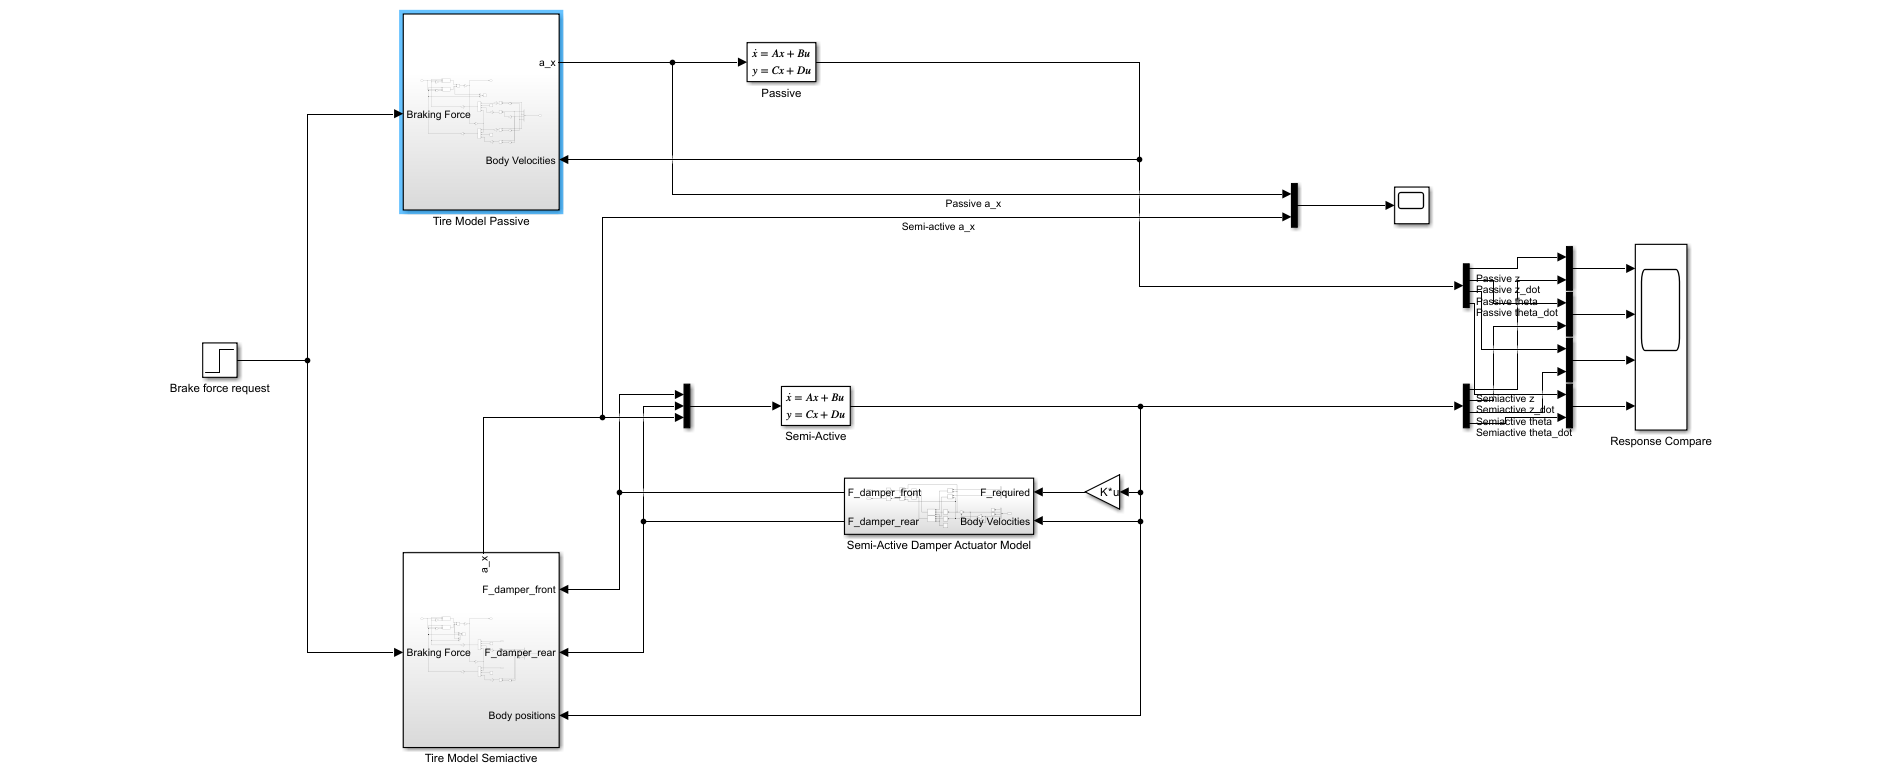
\includegraphics[width=0.9\textwidth]{main_sim.png}
    \caption{Overview of the 2-DOF half-car Simulink simulation framework integrating state-space plant dynamics and closed-loop tire friction saturation logic.}
    \label{fig:main_sim}
\end{figure}

\begin{figure}[htbp]
    \centering
    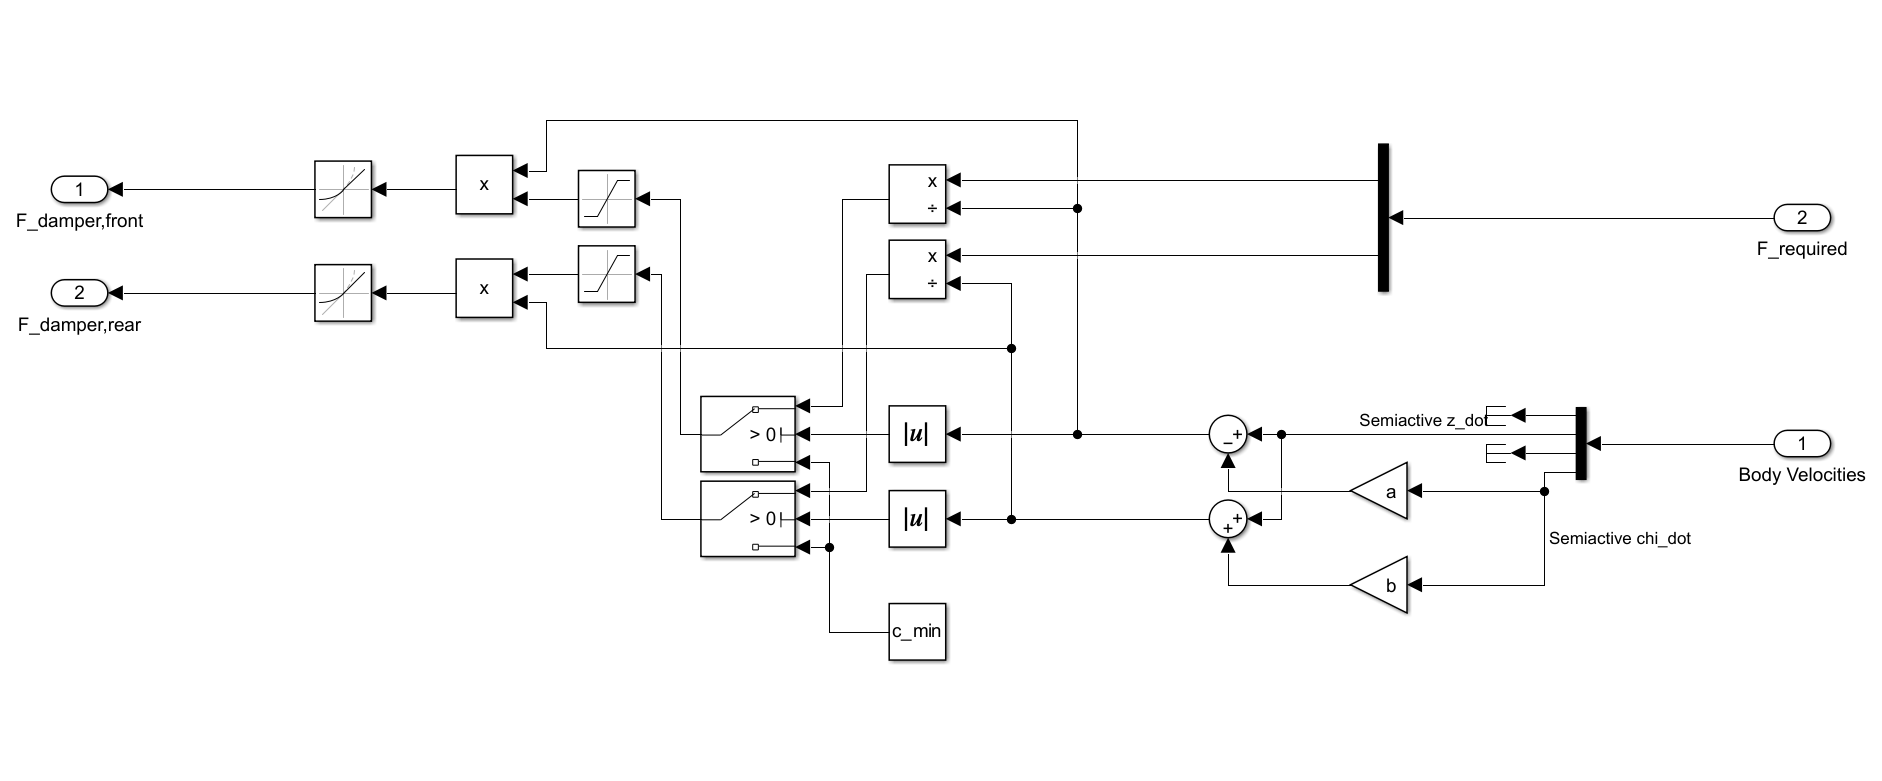
\includegraphics[width=0.9\textwidth]{damper_model.png}
    \caption{Clipped Optimal Damping Realization subsystem incorporating damping saturation, passivity constraints, and valve slew-rate bandwidth limits.}
    \label{fig:damper_model}
\end{figure}

\begin{figure}[htbp]
    \centering
    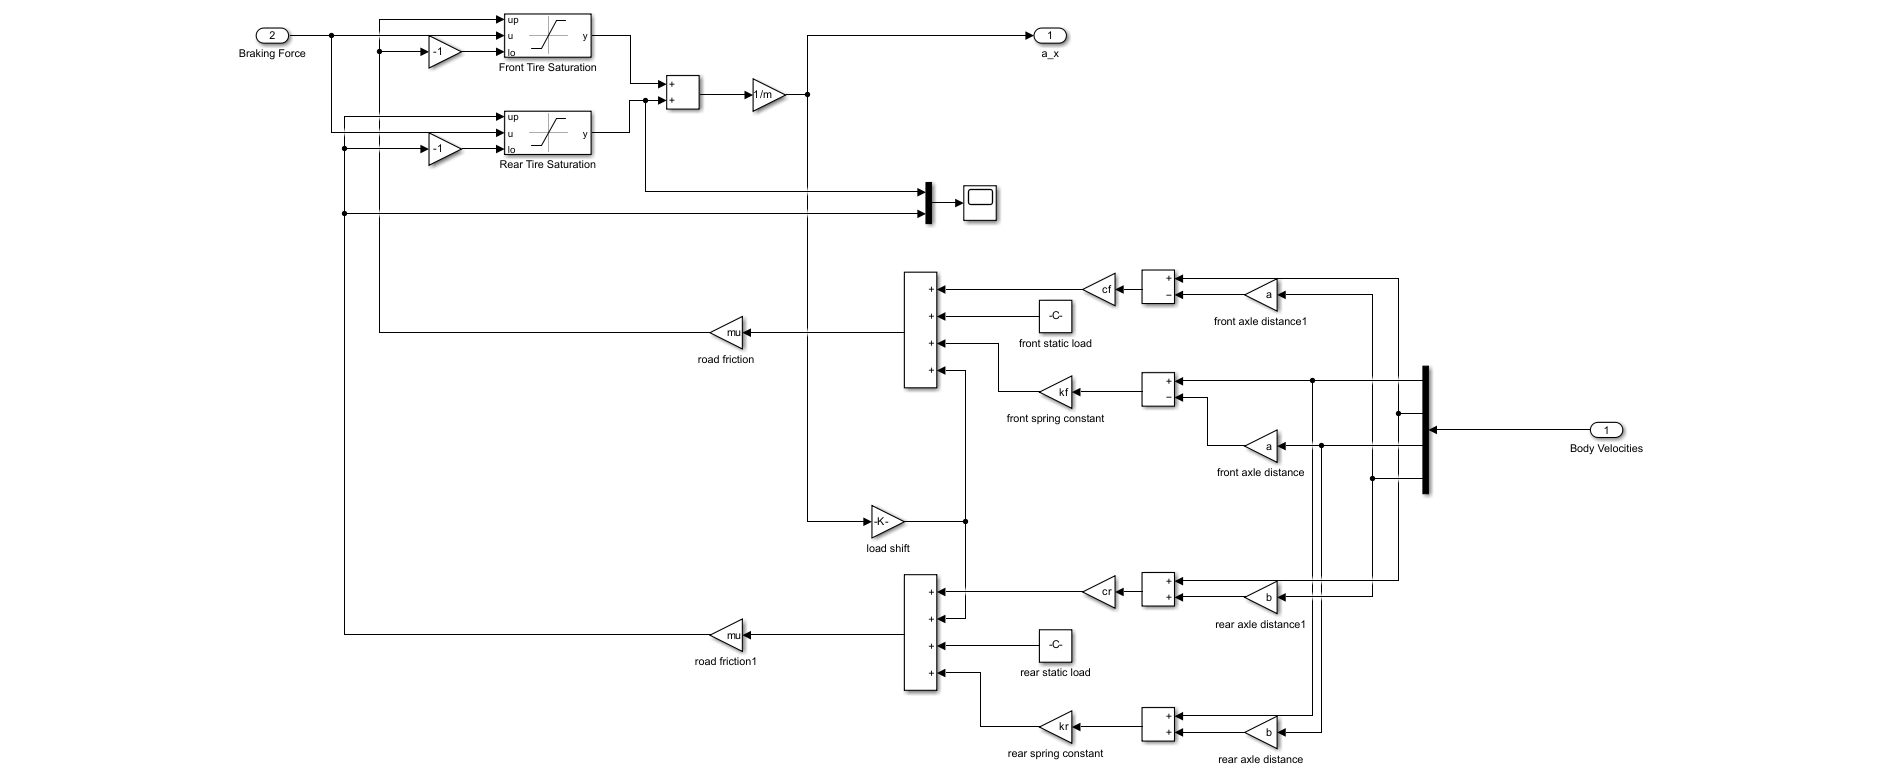
\includegraphics[width=0.9\textwidth]{tiremodelpassive.png}
    \caption{Subsystem architecture for dynamic normal load and friction limit calculation in the passive baseline configuration.}
    \label{fig:tire_passive}
\end{figure}

\begin{figure}[htbp]
    \centering
    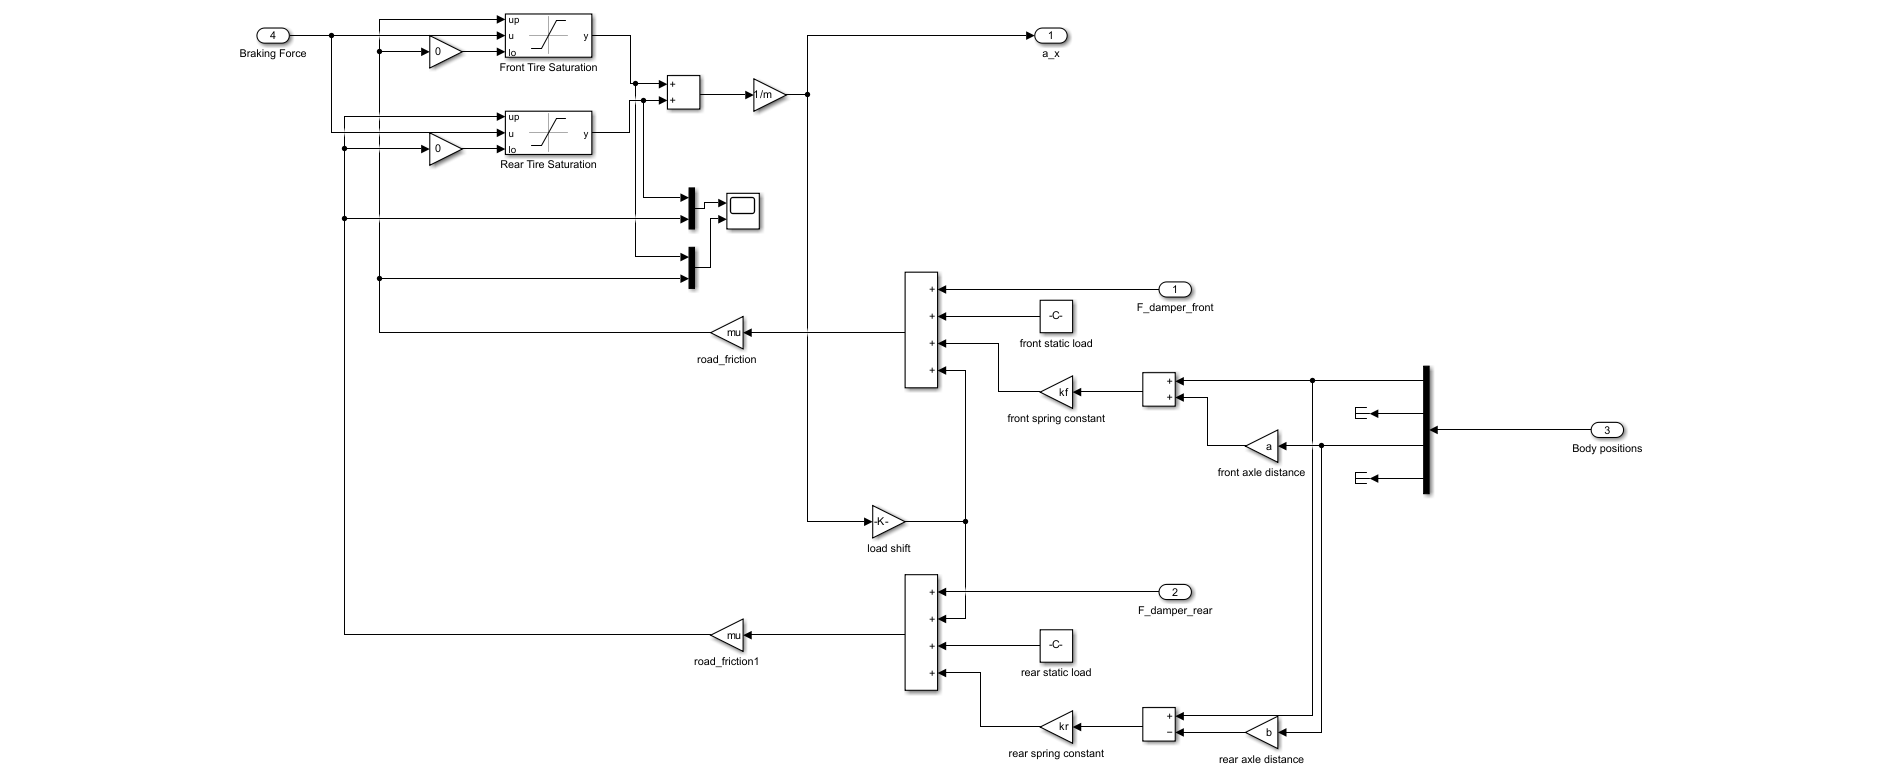
\includegraphics[width=0.9\textwidth]{tiremodelsemi.png}
    \caption{Subsystem architecture incorporating semi-active damper force feedback into dynamic normal load and friction limit calculations.}
    \label{fig:tire_semi}
\end{figure}
\end{document}